% !TeX program = latexmk
% !TeX options = -pdflatex -synctex=1 -interaction=nonstopmode -file-line-error -shell-escape -output-directory="%OUTDIR%" "%DOC%"
\documentclass[aspectratio=169, 10pt]{beamer}
\usepackage[utf8]{vietnam}
\usetheme{Boadilla}
\usecolortheme{default}
\usepackage[x11names]{xcolor}
\usepackage{amsmath,amssymb,fancyhdr}
\usepackage{newpxtext}
\usepackage{newpxmath}
\usefonttheme{serif}
\usefonttheme{professionalfonts}
\usepackage{tikz,tikz-3dplot,tkz-tab}
\usetikzlibrary{arrows,calc,intersections,patterns,angles,shapes.geometric}
\usepackage{booktabs, array, xcolor}
\usepackage{listings}
\usepackage{xcolor}
\usepackage{multicol}

\definecolor{sql_keyword}{HTML}{0000FF}
\definecolor{sql_type}{HTML}{800080}
\definecolor{sql_string}{HTML}{AF0000}
\definecolor{sql_identifier}{HTML}{000000}
\definecolor{sql_bg}{HTML}{FFFFFF}
\definecolor{sql_comment}{HTML}{008000}
\definecolor{sql_num}{HTML}{444444}

\lstset{
    language=SQL,
    backgroundcolor=\color{sql_bg},
    basicstyle=\bfseries\ttfamily\small\color{sql_identifier},
    breakatwhitespace=false,
    breaklines=true,
    captionpos=b,
    commentstyle=\color{sql_comment},
    deletekeywords={DATE},
    escapeinside={\%*}{*)},
    frame=single,
    keepspaces=true,
    keywordstyle=\color{sql_keyword}\bfseries,
    morekeywords={*, SELECT, FROM, WHERE, NOT, IN, GROUP, BY, ORDER, LIMIT, OFFSET, RETURNING, PRIMARY, KEY, FOREIGN, REFERENCES, CONSTRAINT, UNIQUE, INDEX, FUNCTION, TRIGGER, PROCEDURE, REPLACE, LANGUAGE, PLPGSQL, IS, ILIKE, COALESCE, EXISTS, ANY, ARRAY, CASE, WHEN, THEN, ELSE, END, AFTER, BEFORE, FOR, EACH, ROW, EXECUTE, ON, CONFLICT, DO, NOTHING, INTO, DECLARE, BEGIN, RAISE, EXCEPTION, IF, ELSIF, RETURN, RETURNS, VOID, NEW, OLD, NULL, TG_OP, NOW, ASC, DESC, LEFT, JOIN, CAST, LIKE, AS, SET, VALUES},
    classoffset=1,
    morekeywords={UUID, SERIAL, VARCHAR, TEXT, BOOL, TIMESTAMP, INTEGER, REAL, DOUBLE, BIGINT, SMALLINT, JSONB, BOOLEAN, NUMERIC, BIGSERIAL},
    keywordstyle=\color{sql_type}\bfseries,
    classoffset=0,
    numbers=left,
    numbersep=8pt,
    numberstyle=\tiny\bfseries\color{sql_num},
    rulecolor=\color{black},
    showspaces=false,
    showstringspaces=false,
    showtabs=false,
    stringstyle=\color{sql_string},
    tabsize=2,
    xleftmargin=10pt,
    xrightmargin=10pt,
    linewidth=\linewidth
}

\everymath{\displaystyle}
\graphicspath{{Figures/}}
\sloppy
\setbeamerfont{frametitle}{series=\bfseries}
\setbeamerfont{section in toc}{series=\bfseries}
\setbeamerfont{block title}{series=\bfseries}

%------------------------------------------------------------
%This block of code defines the information to appear in the
%Title page
\title[Database Lab – Project 2025.2]
{
    \fontsize{18}{0}{\textcolor{Blue3}{\textbf{Database System Design for\\[0.1cm] An Online Examination and\\[0.1cm] Question Bank Management Platform}}}
}

\author[Phung Minh Phuc]
{\bf 
Group: 01\\ \vspace{0.1cm}
\begin{tabular}{l l}
Phung Minh Phuc & 202417009 \\
Tran Xuan Truong & 202417061 \\
Le Trong Nghia & 202416989 \\
Duong Tuan Phi & 202417001 \\
\end{tabular}
% \begin{tabular}{l l}
%     Phung Minh Phuc & 202417009 \\
%     Tran Xuan Truong & 202417061 \\
% \end{tabular} 
% \hspace{1cm} 
% \begin{tabular}{l l}
%     Le Trong Nghia & 202416989 \\
%     Duong Tuan Phi & 202417001 \\
% \end{tabular}
}
\institute[SoICT-HUST]
{
    \normalsize Hanoi University of Science and Technology
}
\addtobeamertemplate{title page}{%
    \vspace*{0.2cm}
    \begin{flushright}
        
\includegraphics[width=1.2cm]{Images/logo-soict-hust.png}
    \end{flushright}
    \vspace*{-0.5cm}
}{}
\date[\the\year]{\the\year}


\logo{}
\setbeamertemplate{frametitle}{
    \vspace{-0.4cm}
    \begin{beamercolorbox}[wd=\textwidth]{frametitle}
        \begin{minipage}[t]{0.85\textwidth}
            \vspace{0pt}
            \usebeamerfont{frametitle}\insertframetitle\par
            \ifx\insertframesubtitle\@empty\else
                \vspace{0.1cm}
                \usebeamerfont{framesubtitle}\usebeamercolor[fg]{framesubtitle}\insertframesubtitle\par
            \fi
        \end{minipage}\hfill
        \begin{minipage}[t]{0.12\textwidth}
            \raggedleft
            \vspace{0pt}
            
\includegraphics[width=1.2cm]{Images/logo-soict-hust.png}
        \end{minipage}
    \end{beamercolorbox}
    \vspace{0.0cm}
}

\setbeamercolor{title}{parent=date in head/foot}
\hypersetup{
    pdftitle={Database System Design for An Online Examination and Question Bank Management Platform},
    pdfauthor={Phùng Minh Phúc},
    pdfproducer={Microsoft Print to PDF},
    hidelinks,
}
%End of title page configuration block
%------------------------------------------------------------



%------------------------------------------------------------
\AtBeginSection[]
{
  \begin{frame}
    \frametitle{\textbf{Contents}}
    \tableofcontents[currentsection]
  \end{frame}
}

\AtBeginSubsection[]
{
  \begin{frame}
    \frametitle{\textbf{Contents}}
    \tableofcontents[currentsection, currentsubsection]
  \end{frame}
}
%------------------------------------------------------------


\begin{document}
\frame{\titlepage}

\renewcommand{\arraystretch}{1.6} 
\setlength{\tabcolsep}{8pt}     

% ---------------------------------------------------------
\begin{frame}
\frametitle{\textbf{Contents}}
\tableofcontents
\end{frame}
% ---------------------------------------------------------



% ============================================================
%   CHAPTER 1: INTRODUCTION
% ============================================================
\section{Introduction}

\begin{frame}{Background and Motivation}
    \begin{itemize}
        \item Digital education has shifted toward \textbf{integrated platforms} for remote learning and automated assessment
        \item The underlying \textbf{database} is the critical foundation for:
        \begin{itemize}
            \item Data consistency
            \item Operational security
            \item System performance
        \end{itemize}
        \item This project investigates the \textbf{structural design and implementation} of an Online Examination and Question Bank Management Platform using \textbf{PostgreSQL}
    \end{itemize}
\end{frame}


\begin{frame}{Problem Statement}
    Key technical challenges:
    \begin{enumerate}
        \item \textbf{Heterogeneous question formats:} MC, TF, SA, and OE items with multimedia support
        \item \textbf{Hierarchical dependencies:} Parent–child relationships for passage-based questions (Stimulus type)
        \item \textbf{Referential integrity:} Student submissions must map to specific temporal exam states
        \item \textbf{Authorization hierarchies:} Role-based access control (Admin, Teacher, Student)
        \item \textbf{Schema flexibility:} Avoiding data redundancy while supporting diverse data structures
    \end{enumerate}
\end{frame}


\begin{frame}{Project Objectives}
    \begin{enumerate}
        \item \textbf{Identity \& Access Management (IAM):} Role-based delineation of Admin, Teacher, Student
        \item \textbf{Academic Organization:} Student–Teacher interactions mediated through classroom entities
        \item \textbf{Polymorphic Question Bank:} Complex metadata, difficulty stratification, randomized components
        \item \textbf{Assessment Engine:} JSONB-based dynamic scoring, automated grading, analytical reporting
    \end{enumerate}
    \vspace{0.3cm}
    \begin{block}{Technology Stack}
        PostgreSQL $\bullet$ Python (FastAPI + psycopg2) $\bullet$ Next.js (React) $\bullet$ UUID + JSONB
    \end{block}
\end{frame}


\begin{frame}{System Overview}
    \begin{columns}[T]
        \begin{column}{0.48\textwidth}
            \textbf{Methodology:}
            \begin{itemize}
                \item Strict database normalization principles
                \item UUID for secure external exposure
                \item TIMESTAMP logging for auditability
                \item Hybrid normalization + strategic denormalization
            \end{itemize}
        \end{column}
        \begin{column}{0.48\textwidth}
            \textbf{4 Functional Modules:}
            \begin{enumerate}
                \item Identity Management
                \item Classroom Organization
                \item Hierarchical Question Bank
                \item Assessment Engine
            \end{enumerate}
        \end{column}
    \end{columns}
    \vspace{0.3cm}
    \begin{block}{Project Resources}
        \footnotesize
        GitHub: \url{https://github.com/PhungMinhPhuc/question-dataset}\\
        DB Backup: \url{https://drive.google.com/drive/folders/1SPMrp4qBzDp1KWkO36wYqUqM9LMyFtr_}
    \end{block}
\end{frame}



% ============================================================
%   CHAPTER 2: DATABASE DESIGN AND SCHEMA ANALYSIS
% ============================================================
\section{Database Design and Schema Analysis}

% --- ERD ---
\subsection{Entity-Relationship Diagram}
\begin{frame}{Entity-Relationship Diagram (ERD)}
    \begin{center}
        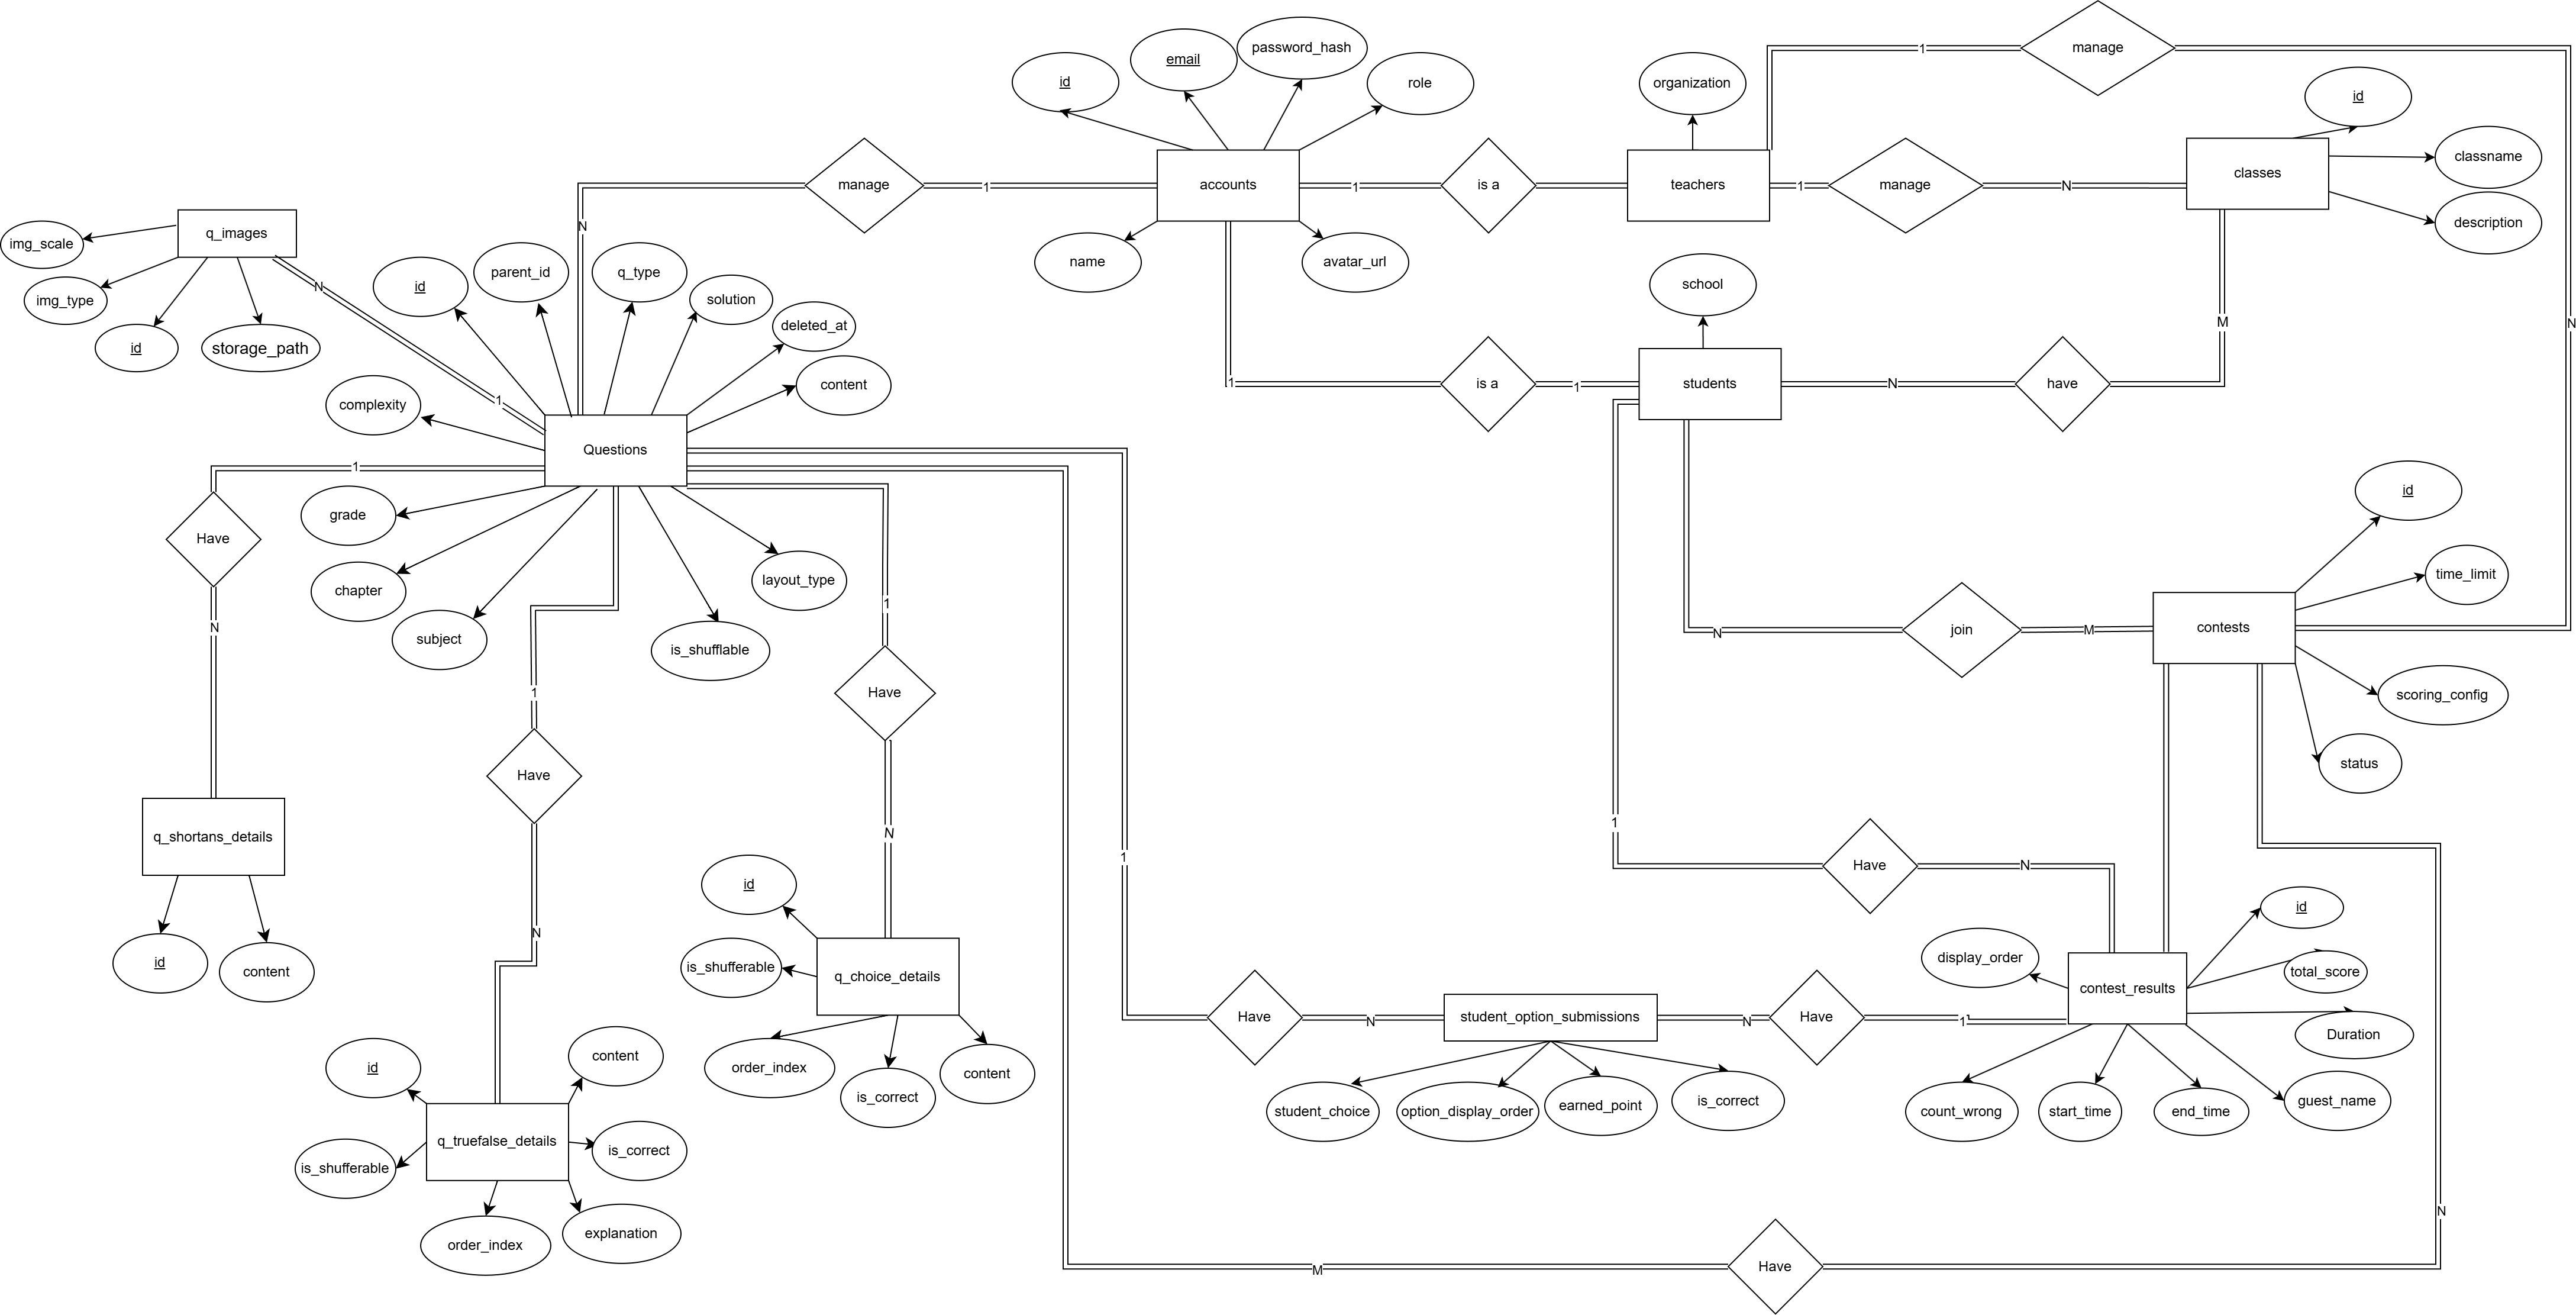
\includegraphics[width=0.95\textwidth]{Entity_Relationship_Diagram.jpg}
    \end{center}
\end{frame}


% --- Relational Schema ---
\subsection{Relational Schema}
\begin{frame}{Relational Schema}
    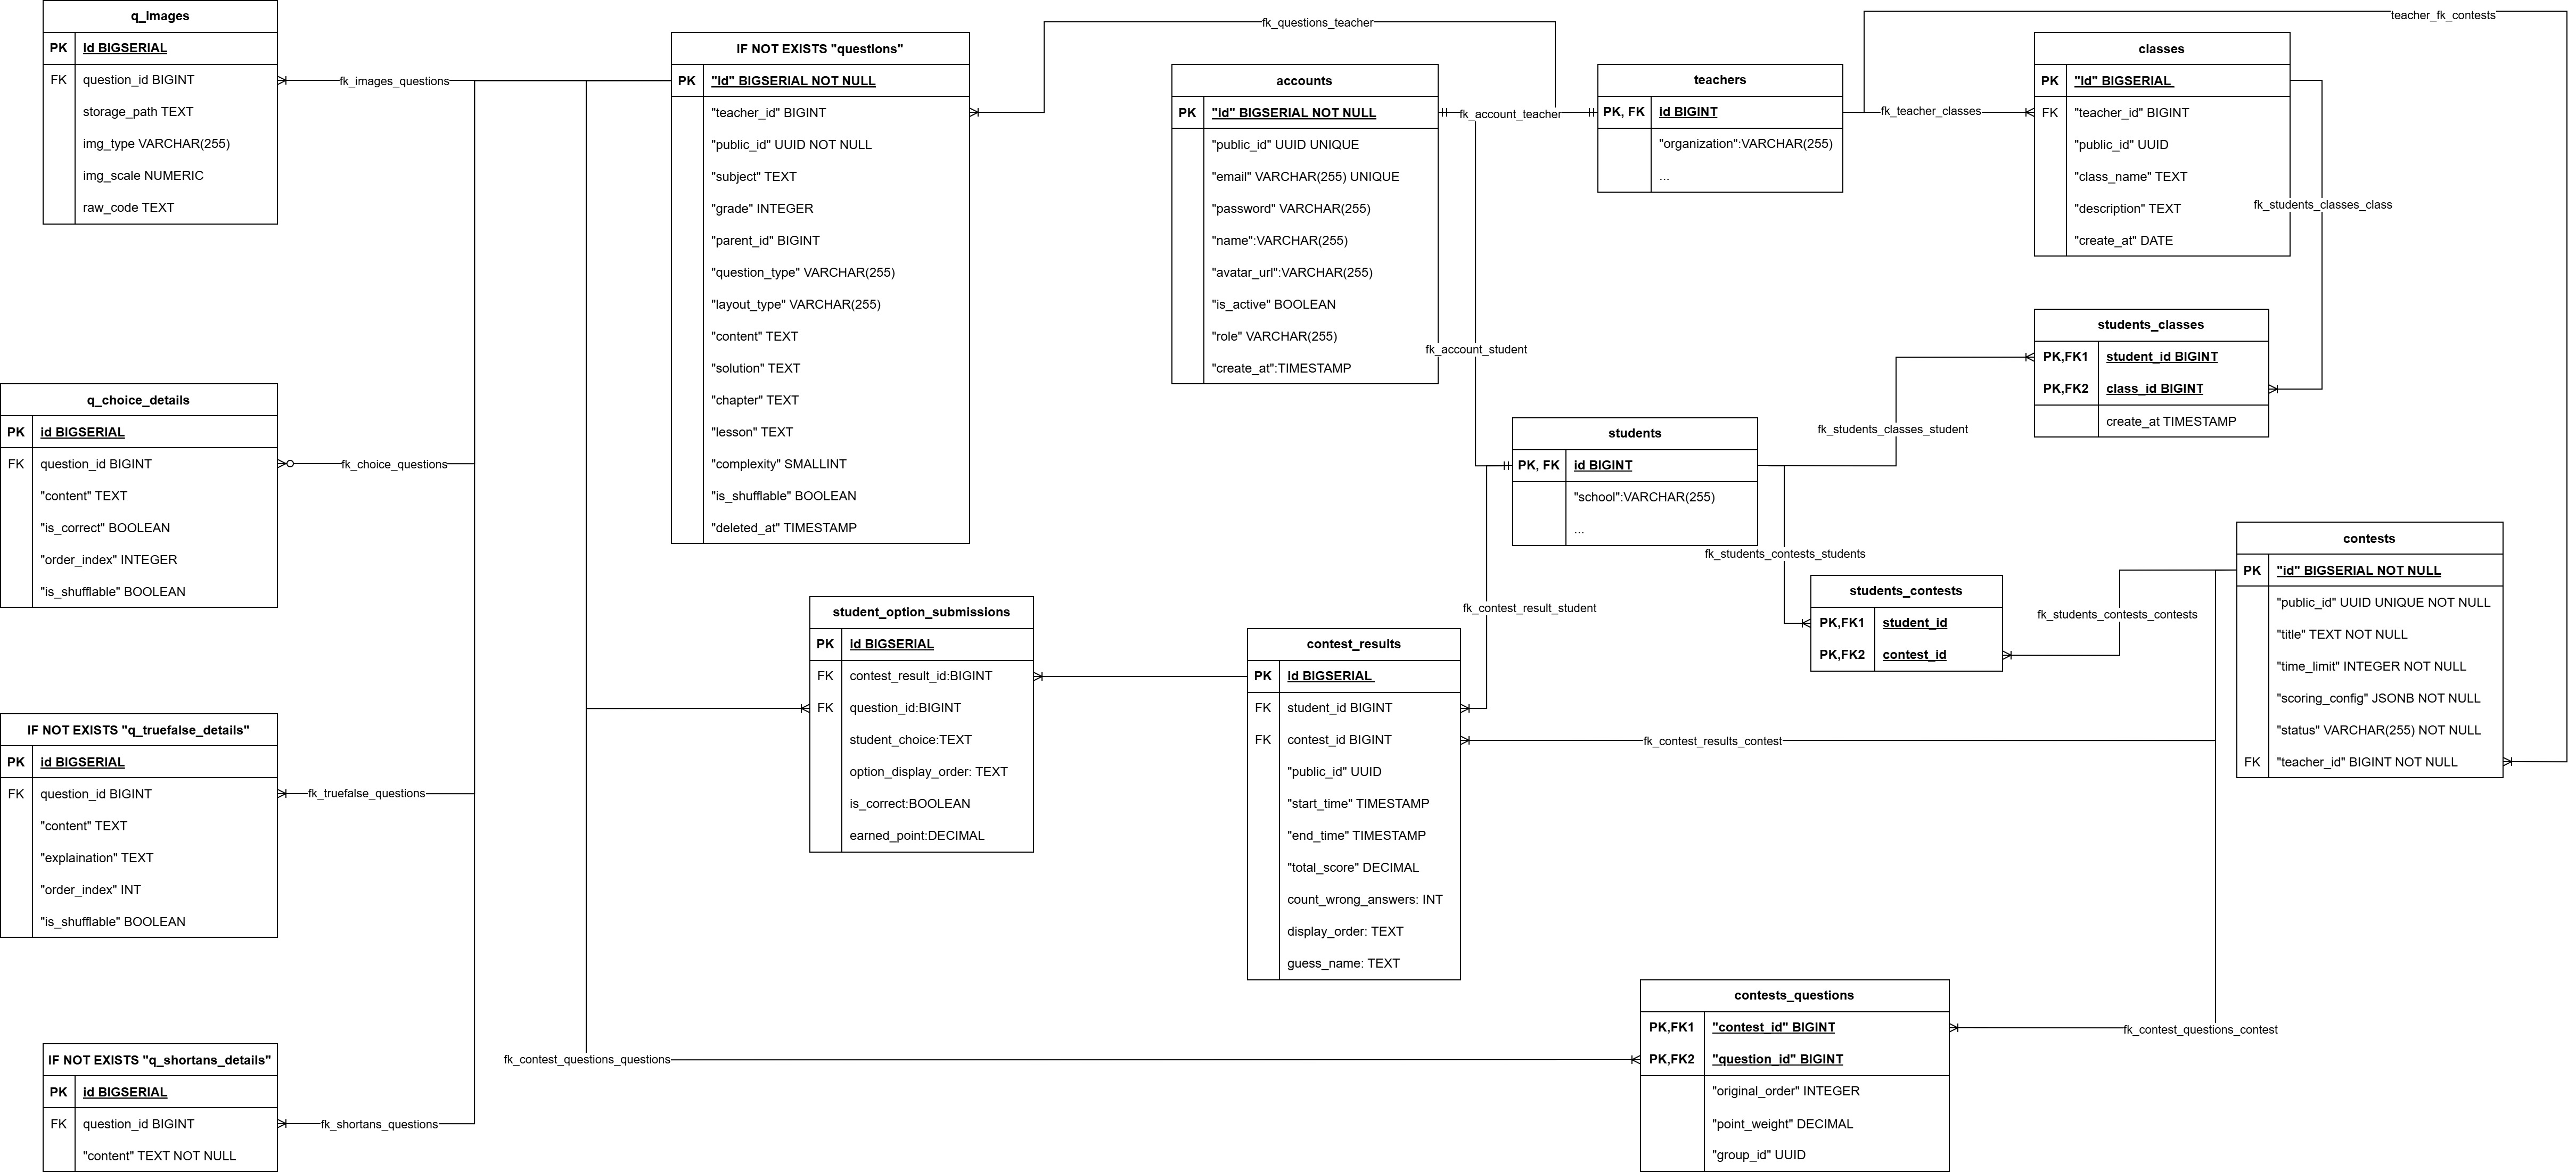
\includegraphics[width=\textwidth]{Relational_Schema.jpg}
\end{frame}


% --- Design Modules ---
\subsection{Architectural Design Decisions}

\begin{frame}{Module 1: Identity and Access Management}
    \begin{columns}[T]
        \begin{column}{0.55\textwidth}
            \begin{itemize}
                \item \texttt{accounts} table: central identity registry
                \item \textbf{Specialization pattern:} 1-to-1 relationship to \texttt{teachers} and \texttt{students}
                \item Avoids sparse tables by decoupling role-specific data
                \item FK constraints ensure no orphan profiles
            \end{itemize}
        \end{column}
        \begin{column}{0.4\textwidth}
            \centering
            \small
            \begin{tabular}{|l|l|}
                \hline
                \textbf{Table} & \textbf{Key Fields} \\ \hline
                \texttt{accounts} & id, email, role \\ \hline
                \texttt{teachers} & id (FK), org \\ \hline
                \texttt{students} & id (FK), school \\ \hline
            \end{tabular}
        \end{column}
    \end{columns}
\end{frame}


\begin{frame}{Module 2: Classroom \& Enrollment}
    \begin{itemize}
        \item \textbf{1-to-Many:} One teacher owns many classes
        \item \textbf{Many-to-Many:} Students $\leftrightarrow$ Classes via junction table \texttt{students\_classes}
        \item \texttt{public\_id} (UUID) enables secure class sharing/joining
        \item Content filtering based on class membership
    \end{itemize}
    \vspace{0.3cm}
    \centering
    \small
    \begin{tabular}{|l|l|p{6cm}|}
        \hline
        \textbf{Table} & \textbf{Type} & \textbf{Purpose} \\ \hline
        \texttt{classes} & Entity & Pedagogical unit owned by a teacher \\ \hline
        \texttt{students\_classes} & Junction & M:N enrollment with timestamp \\ \hline
    \end{tabular}
\end{frame}


\begin{frame}{Module 3: The Polymorphic Question Bank}
    \begin{columns}[T]
        \begin{column}{0.55\textwidth}
            \begin{itemize}
                \item \texttt{questions}: polymorphic hub with common metadata
                \item \textbf{Self-referencing FK} (\texttt{parent\_id}) for hierarchical Stimulus questions
                \item \textbf{Horizontal partitioning:} type-specific detail tables
                \item \texttt{q\_images}: decoupled multimedia support
            \end{itemize}
        \end{column}
        \begin{column}{0.42\textwidth}
            \centering
            \small
            \begin{tabular}{|l|}
                \hline
                \textbf{Detail Tables} \\ \hline
                \texttt{q\_choice\_details} (MC) \\ \hline
                \texttt{q\_truefalse\_details} (TF) \\ \hline
                \texttt{q\_shortans\_details} (SA) \\ \hline
                \texttt{q\_images} (Media) \\ \hline
            \end{tabular}
        \end{column}
    \end{columns}
\end{frame}


\begin{frame}{Design Rationale: Strategic Denormalization}
    \begin{block}{Problem}
        Fully normalizing \texttt{subject}, \texttt{grade}, \texttt{chapter}, \texttt{lesson} into separate tables would require deeply nested JOINs
    \end{block}
    \vspace{0.2cm}
    \begin{block}{Solution}
        Store as TEXT in \texttt{questions} table, constrained by a structured JSON curriculum file (Single Source of Truth)
    \end{block}
    \vspace{0.2cm}
    \textbf{Advantages:}
    \begin{itemize}
        \item \textbf{Reduced Query Complexity:} Eliminates nested JOINs for filtering
        \item \textbf{Maintainability:} Curriculum updates only require modifying the JSON file — no schema migrations needed
    \end{itemize}
\end{frame}


\begin{frame}{Module 4: Assessment \& Result Tracking}
    \begin{itemize}
        \item \texttt{contests}: exam parameters (time limit, status, JSONB scoring config)
        \item \texttt{contests\_questions}: junction table that \textbf{snapshots} point weights at exam creation time
        \item \texttt{contest\_results}: aggregated performance metrics per attempt
        \item \texttt{student\_option\_submissions}: granular log of every response
        \begin{itemize}
            \item Stores \texttt{option\_display\_order} for audit trail
            \item Stores raw \texttt{student\_choice} for review
        \end{itemize}
    \end{itemize}
\end{frame}


% --- Detailed Tables ---
\subsection{Database Tables}

% 1. Accounts
\begin{frame}{1. \texttt{Accounts}}
    \centering
    \footnotesize
    \begin{tabular}{|l|l|p{8cm}|}
        \hline
        \textbf{Attribute} & \textbf{Datatype} & \textbf{Description} \\ \hline
        \texttt{id} & Bigserial (PK) & Auto-generated unique identifier of an account\\ \hline
        \texttt{public\_id} & UUID (UQ) & Public unique identifier used externally\\ \hline
        \texttt{email} & Varchar & User email address\\ \hline
        \texttt{password} & Varchar & Encrypted password\\ \hline
        \texttt{name} & Varchar & Full name of the user\\ \hline
        \texttt{avatar\_url} & Varchar & URL of the user profile picture\\ \hline
        \texttt{is\_active} & Boolean & Account status (active/inactive)\\ \hline
        \texttt{role} & Varchar & User role: Admin, Teacher, or Student\\ \hline
        \texttt{create\_at} & Timestamp & Account creation timestamp\\ \hline
    \end{tabular}
    \vspace{0.2cm}
    \begin{itemize}
        \item Centralized identity management table.
        \item \texttt{public\_id} prevents exposing sequential IDs in API routes.
    \end{itemize}
\end{frame}


% 2. Teachers
\begin{frame}{2. \texttt{Teachers}}
    \centering
    \small
    \begin{tabular}{|l|l|p{8cm}|}
        \hline
        \textbf{Attribute} & \textbf{Datatype} & \textbf{Description} \\ \hline
        \texttt{id} & Bigint (PK, FK) & References the corresponding account ID\\ \hline
        \texttt{organization} & Varchar & Institution or department affiliation\\ \hline
        \texttt{...} & ... & ...\\ \hline
    \end{tabular}
    \vspace{0.3cm}
    \begin{itemize}
        \item Extended profile specifically for educators.
        \item Enforces 1-to-1 relationship with the \texttt{Accounts} table.
        \item Shared fields (name, avatar\_url) are stored in \texttt{Accounts}.
    \end{itemize}
\end{frame}


% 3. Students
\begin{frame}{3. \texttt{Students}}
    \centering
    \small
    \begin{tabular}{|l|l|p{8cm}|}
        \hline
        \textbf{Attribute} & \textbf{Datatype} & \textbf{Description} \\ \hline
        \texttt{id} & Bigint (PK, FK) & References the corresponding account ID\\ \hline
        \texttt{school} & Varchar & Name of the student's school\\ \hline
        \texttt{...} & ... & ...\\ \hline
    \end{tabular}
    \vspace{0.3cm}
    \begin{itemize}
        \item Extended profile specifically for examinees.
        \item Allows segregation of student metadata from authentication credentials.
        \item Shared fields (name, avatar\_url) are stored in \texttt{Accounts}.
    \end{itemize}
\end{frame}


% 4. Classes
\begin{frame}{4. \texttt{Classes}}
    \centering
    \small
    \begin{tabular}{|l|l|p{8cm}|}
        \hline
        \textbf{Attribute} & \textbf{Datatype} & \textbf{Description} \\ \hline
        \texttt{id} & Bigserial (PK) & Auto-generated id of each class\\ \hline
        \texttt{teacher\_id} & Bigint (FK) & Id of the teacher in charge of the class\\ \hline
        \texttt{public\_id} & UUID & Auto-generated UUID for secure sharing\\ \hline
        \texttt{class\_name} & Text & Display name of the class\\ \hline
        \texttt{description} & Text & Optional description or syllabus overview\\ \hline
        \texttt{create\_at} & Timestamp & Timestamp when user created the class\\ \hline
    \end{tabular}
    \vspace{0.3cm}
    \begin{itemize}
        \item Logical grouping entity for students.
        \item Strictly owned and managed by a single \texttt{teacher\_id}.
    \end{itemize}
\end{frame}


% 5. Students_Classes
\begin{frame}{5. \texttt{Students\_Classes}}
    \centering
    \small
    \begin{tabular}{|l|l|p{8cm}|}
        \hline
        \textbf{Attribute} & \textbf{Datatype} & \textbf{Description} \\ \hline
        \texttt{student\_id} & Bigint (PK, FK) & Foreign Key points to student's Id\\ \hline
        \texttt{class\_id} & Bigint (PK, FK) & Foreign Key points to class's Id\\ \hline
        \texttt{create\_at} & Timestamp & Timestamp when student joins class\\ \hline
    \end{tabular}
    \vspace{0.3cm}
    \begin{itemize}
        \item Junction table resolving the Many-to-Many relationship between Students and Classes.
        \item Composite Primary Key ensures a student cannot join the same class twice.
    \end{itemize}
\end{frame}


% 6. Questions
\begin{frame}{6. \texttt{Questions}}
    \centering
    \scriptsize
    \begin{tabular}{|l|l|p{8cm}|}
        \hline
        \textbf{Attribute} & \textbf{Datatype} & \textbf{Description} \\ \hline
        \texttt{id} & Bigserial (PK) & Auto-generated unique identifier\\ \hline
        \texttt{teacher\_id} & Bigint (FK) & References Teachers(id)\\ \hline
        \texttt{public\_id} & UUID (UQ) & Public unique identifier\\ \hline
        \texttt{subject} & Text & Subject name\\ \hline
        \texttt{grade} & Integer & Grade level\\ \hline
        \texttt{parent\_id} & Bigint (FK) & References parent question (Questions(id))\\ \hline
        \texttt{question\_type} & Varchar & e.g., MC, TF, SA,...\\\hline
        \texttt{layout\_type} & Varchar & Layout configuration\\\hline
        \texttt{content} & Text & The question text\\ \hline
        \texttt{solution} & Text & Official solution/explanation\\\hline
        \texttt{chapter} & Text & Chapter name\\\hline
        \texttt{lesson} & Text & Lesson name\\\hline
        \texttt{complexity} & Smallint & Difficulty level\\ \hline
        \texttt{is\_shufflable} & Boolean & Indicates if components can be shuffled\\ \hline
        \texttt{deleted\_at} & Timestamp & Soft delete timestamp\\ \hline
    \end{tabular}
    \vspace{0.1cm}
    \begin{itemize}
        \item Core polymorphic table storing universal properties of all assessment items.
    \end{itemize}
\end{frame}


% 7. Q_Images
\begin{frame}{7. \texttt{Q\_Images}}
    \centering
    \small
    \begin{tabular}{|l|l|p{8cm}|}
        \hline
        \textbf{Attribute} & \textbf{Datatype} & \textbf{Description} \\ \hline
        \texttt{id} & Bigserial (PK) & Auto-generated id\\ \hline
        \texttt{question\_id} & Bigint (FK) & Foreign key points to question's id\\ \hline
        \texttt{storage\_path} & Text & File path or URL of the image\\ \hline
        \texttt{img\_type} & Varchar & Format of the image (png, jpg)\\ \hline
        \texttt{img\_scale} & Decimal & Rendering scale coefficient\\ \hline
        \texttt{raw\_code} & Text & Optional base64 or LaTeX raw representation\\ \hline
    \end{tabular}
    \vspace{0.3cm}
    \begin{itemize}
        \item Extends the \texttt{Questions} table to support rich multimedia.
        \item 1-to-N relationship allows multiple images per question.
    \end{itemize}
\end{frame}


% 8. Q_Choice_Details
\begin{frame}{8. \texttt{Q\_Choice\_Details}}
    \centering
    \small
    \begin{tabular}{|l|l|p{8cm}|}
        \hline
        \textbf{Attribute} & \textbf{Datatype} & \textbf{Description} \\ \hline
        \texttt{id} & Bigserial (PK) & Auto-generated id\\ \hline
        \texttt{question\_id} & Bigint (FK) & Links back to the parent question\\ \hline
        \texttt{content} & Text & The text of the choice option\\ \hline
        \texttt{is\_correct} & Boolean & True if this is the correct answer\\\hline 
        \texttt{order\_index} & Int & Default display order\\ \hline
        \texttt{is\_shufflable} & Boolean & Allows anchoring options like "All of the above"\\ \hline
    \end{tabular}
    \vspace{0.3cm}
    \begin{itemize}
        \item Sub-table specific to Multiple Choice questions.
        \item Contains the granular pool of possible answers.
    \end{itemize}
\end{frame}


% 9. Q_TrueFalse_Details
\begin{frame}{9. \texttt{Q\_TrueFalse\_Details}}
    \centering
    \small
    \begin{tabular}{|l|l|p{8cm}|}
        \hline
        \textbf{Attribute} & \textbf{Datatype} & \textbf{Description} \\ \hline
        \texttt{id} & Bigserial (PK) & Auto-generated id\\ \hline
        \texttt{question\_id} & Bigint (FK) & Links back to the parent question\\ \hline
        \texttt{content} & Text & Statement to be evaluated\\ \hline
        \texttt{is\_correct} & Boolean & The boolean truth value of the statement\\ \hline
        \texttt{explaination} & Text & Pedagogical explanation for the correct answer\\ \hline
        \texttt{order\_index} & Int & Default display order\\ \hline
        \texttt{is\_shufflable} & Boolean & Whether this specific row can be shuffled\\\hline
    \end{tabular}
    \vspace{0.3cm}
    \begin{itemize}
        \item Sub-table for True/False questions.
        \item Includes explanations for post-exam review.
    \end{itemize}
\end{frame}


% 10. Q_ShortAns_Details
\begin{frame}{10. \texttt{Q\_ShortAns\_Details}}
    \centering
    \small
    \begin{tabular}{|l|l|p{8cm}|}
        \hline
        \textbf{Attribute} & \textbf{Datatype} & \textbf{Description} \\ \hline
        \texttt{id} & Bigserial (PK) & Auto-generated id\\ \hline
        \texttt{question\_id} & Bigint (FK) & Links back to the parent question\\ \hline
        \texttt{content} & Text & The exact valid text string for automated grading\\ \hline
    \end{tabular}
    \vspace{0.3cm}
    \begin{itemize}
        \item Sub-table for Fill-in-the-blank or Short Answer questions.
        \item Multiple valid variations can be inserted per question.
    \end{itemize}
\end{frame}


% 11. Contests
\begin{frame}{11. \texttt{Contests}}
    \centering
    \small
    \begin{tabular}{|l|l|p{8cm}|}
        \hline
        \textbf{Attribute} & \textbf{Datatype} & \textbf{Description} \\ \hline
        \texttt{id} & Bigserial (PK) & Contest identifier\\ \hline
        \texttt{class\_id} & Bigint & Class identifier\\ \hline
        \texttt{public\_id} & UUID (UQ) & Public unique identifier\\ \hline
        \texttt{title} & Text & Contest title\\ \hline
        \texttt{time\_limit} & Integer & Duration limit in minutes\\ \hline
        \texttt{scoring\_config} & JSONB & JSON configuration for scoring\\ \hline
        \texttt{status} & Varchar & Status (`active', `inactive')\\ \hline
    \end{tabular}
    \vspace{0.3cm}
    \begin{itemize}
        \item Core entity defining an examination session.
        \item \texttt{scoring\_config} natively utilizes PostgreSQL JSONB for flexible rulesets.
    \end{itemize}
\end{frame}


% 12. Contests_Questions
\begin{frame}{12. \texttt{Contests\_Questions}}
    \centering
    \small
    \begin{tabular}{|l|l|p{8cm}|}
        \hline
        \textbf{Attribute} & \textbf{Datatype} & \textbf{Description} \\ \hline
        \texttt{contest\_id} & Bigint (FK) & References Contests(id)\\ \hline
        \texttt{question\_id} & Bigint (FK) & References Questions(id)\\ \hline
        \texttt{original\_order} & Integer & Display order of the question\\ \hline
        \texttt{point\_weight} & Numeric & Points assigned to the question\\ \hline
    \end{tabular}
    \vspace{0.3cm}
    \begin{itemize}
        \item Junction table linking questions to a specific contest.
        \item Snapshots point weights at exam creation, protecting contest integrity.
    \end{itemize}
\end{frame}


% 13. Students_Contests
\begin{frame}{13. \texttt{Students\_Contests}}
    \centering
    \small
    \begin{tabular}{|l|l|p{8cm}|}
        \hline
        \textbf{Attribute} & \textbf{Datatype} & \textbf{Description} \\ \hline
        \texttt{student\_id} & Bigint (FK) & References Students(id)\\ \hline
        \texttt{contest\_id} & Bigint (FK) & References Contests(id)\\ \hline
    \end{tabular}
    \vspace{0.3cm}
    \begin{itemize}
        \item Explicit access control matrix.
        \item Allows subset of students in a class to take makeup exams.
    \end{itemize}
\end{frame}


% 14. Contest_Results
\begin{frame}{14. \texttt{Contest\_Results}}
    \centering
    \footnotesize
    \begin{tabular}{|l|l|p{8cm}|}
        \hline
        \textbf{Attribute} & \textbf{Datatype} & \textbf{Description} \\ \hline
        \texttt{id} & Bigserial (PK) & Result identifier\\ \hline
        \texttt{student\_id} & Bigint (FK) & References Students(id)\\ \hline
        \texttt{contest\_id} & Bigint (FK) & References Contests(id)\\ \hline
        \texttt{start\_time} & Timestamp & Start timestamp\\ \hline
        \texttt{end\_time} & Timestamp & End timestamp\\ \hline
        \texttt{total\_score} & Numeric & Total calculated score\\ \hline
        \texttt{count\_wrong\_answers}& Integer & Number of incorrect answers\\ \hline
        \texttt{display\_order} & Text & Stored display order\\ \hline
        \texttt{guest\_name} & Text & Guest name who took the exam without an account\\ \hline
    \end{tabular}
    \vspace{0.3cm}
    \begin{itemize}
        \item Immutable snapshot of a completed or ongoing exam session.
        \item \texttt{display\_order} allows deterministic recreation of the test UI for audits.
    \end{itemize}
\end{frame}


% 15. Student_Option_Submissions
\begin{frame}{15. \texttt{Student\_Option\_Submissions}}
    \centering
    \small
    \begin{tabular}{|l|l|p{8cm}|}
        \hline
        \textbf{Attribute} & \textbf{Datatype} & \textbf{Description} \\ \hline
        \texttt{id} & Bigserial (PK) & Submission identifier\\ \hline
        \texttt{contest\_result\_id} & Bigint (FK) & References Contest\_Results(id)\\ \hline
        \texttt{question\_id} & Bigint (FK) & References Questions(id)\\ \hline
        \texttt{student\_choice} & Text & The choice made by the student\\ \hline
        \texttt{option\_display\_order}& Text & Display order presented\\ \hline
        \texttt{is\_correct} & Boolean & Whether the choice was correct\\ \hline
        \texttt{earned\_point} & Numeric& Points earned for this submission\\ \hline
    \end{tabular}
    \vspace{0.3cm}
    \begin{itemize}
        \item Granular record of every single action taken during the exam.
    \end{itemize}
\end{frame}



% ============================================================
%   CHAPTER 3: SQL STATEMENTS AND PERFORMANCE ANALYSIS
% ============================================================
\section{SQL Statements and Performance Analysis}

% ---- Authentication & Profile ----
\subsection{Authentication \& Profile Queries}

\begin{frame}[fragile]{Q1 -- Check login information}
    \begin{lstlisting}
SELECT * FROM accounts 
WHERE email = 'teacher1@email.com' AND is_active = true;
-- Password verification is handled at the application level using a Python function
    \end{lstlisting}
\end{frame}


\begin{frame}[fragile]{Q2 -- Retrieve full user profile with role-specific details}
    \begin{lstlisting}
SELECT a.id, a.email, a.role, a.name, a.avatar_url,
       t.organization, s.school
FROM accounts a
LEFT JOIN teachers t ON a.id = t.id AND a.role = 'teacher'
LEFT JOIN students s ON a.id = s.id AND a.role = 'student'
WHERE a.id = 123456;
    \end{lstlisting}
\end{frame}


\begin{frame}[fragile]{Q3--Q6 -- Account CRUD Operations}
    \begin{lstlisting}
-- Q3: Create a new user account
INSERT INTO accounts (email, password, role, name) 
VALUES ('teacher@email.com', 'password', 'teacher', 'Teacher name')
RETURNING id;

-- Q4: Create teacher/student profile
INSERT INTO teachers (id, organization) VALUES (123456, 'SoICT-HUST');

-- Q5: Update user profile
UPDATE accounts SET name = 'New Name' WHERE id = 123456;

-- Q6: Change password
UPDATE accounts SET password = 'new_hashed_password' WHERE id = 123456;
    \end{lstlisting}
\end{frame}


% ---- Data Upload & Modification ----
\subsection{Data Upload \& Modification Queries}

\begin{frame}[fragile]{Q7 -- Upload a new question}
    \begin{lstlisting}
INSERT INTO questions (
    teacher_id, public_id, subject, grade, parent_id,
    question_type, layout_type, content, solution,
    chapter, lesson, complexity, is_shufflable
)
VALUES (
    123456, '1b95845a...', 'Physics', '12', NULL,
    'mc', 'normal', 'Question Content...', 
    'Detailed Solution...', 'Chapter 1', 'Lesson 1', 1, TRUE
)
RETURNING id;
    \end{lstlisting}
\end{frame}


\begin{frame}[fragile]{Q8--Q12 -- Question Detail Operations}
    \begin{lstlisting}
-- Q8: Upload question image
INSERT INTO q_images (question_id, storage_path, img_type, img_scale) 
VALUES (123456, '/static/img.png', 'png', 1.0);

-- Q9: Upload MC options
INSERT INTO q_choice_details (question_id, content, is_correct, order_index, is_shufflable) 
VALUES (123456, 'Option A', TRUE, 1, TRUE),
       (123456, 'Option B', FALSE, 2, TRUE);

-- Q10: Update content
UPDATE questions SET content = 'New...', complexity = 4 WHERE id = 123456;

-- Q11: Update option
UPDATE q_choice_details SET content = 'New Option' WHERE id = 11223344;

-- Q12: Update image scale
UPDATE q_images SET img_scale = 0.8 WHERE question_id = 123456;
    \end{lstlisting}
\end{frame}


\begin{frame}[fragile]{Q13--Q15 -- Question Deletion}
    \begin{lstlisting}
-- Q13: Soft delete question
UPDATE questions SET deleted_at = NOW() 
WHERE id = 111 AND teacher_id = 81; 
-- Prevent teacher A try to delete teacher B question

-- Q14: Restore soft-deleted question
UPDATE questions SET deleted_at = NULL 
WHERE id = 111 AND teacher_id = 81;

-- Q15: Permanently delete question
DELETE FROM questions WHERE id = 11539 AND teacher_id = 81;
    \end{lstlisting}
\end{frame}


% ---- Question Bank Managing ----
\subsection{Question Bank Managing Queries}

\begin{frame}[fragile]{Q16 -- Count questions with hierarchical text search}
    \begin{lstlisting}
SELECT COUNT(*) as total 
FROM questions q 
WHERE q.deleted_at IS NULL 
AND q.parent_id IS NULL 
AND q.teacher_id = 81 
AND q.subject = 'Physics' AND q.grade = 12 
AND (q.content ILIKE '%BJT transistor%' OR EXISTS 
    (SELECT 1 FROM questions child 
    WHERE child.parent_id = q.id 
    AND child.content ILIKE '%BJT transistor%'));
    \end{lstlisting}
\end{frame}


\begin{frame}[fragile]{Q17 -- Paginated Question Retrieval}
    \begin{lstlisting}
-- Q17: First page with pagination
SELECT q.*, t.name AS teacher_name
FROM questions q LEFT JOIN accounts t ON q.teacher_id = t.id
WHERE q.deleted_at IS NULL AND q.parent_id IS NULL AND q.teacher_id = 81
ORDER BY q.id DESC LIMIT 20 OFFSET 0;
    \end{lstlisting}
\end{frame}


\begin{frame}[fragile]{Q18--Q20 -- Batch Fetching Relations}
\begin{lstlisting}
-- Q18: Question images
SELECT question_id, storage_path, img_scale 
FROM q_images WHERE question_id IN (1000, 1010, 1005);

-- Q19: Question options
SELECT id, question_id, content, is_correct 
FROM q_choice_details WHERE question_id IN (4, 5);

-- Q20: Child questions (stimulus/group)
SELECT id, parent_id, question_type, content 
FROM questions WHERE parent_id IN (1431, 481, 502) ORDER BY id ASC;
\end{lstlisting}
    \vspace{0.2cm}
    \begin{itemize}
        \item Queries 18, 19, and 20 demonstrate a batch query optimization technique (using the \texttt{IN (...)} clause) to resolve the $N+1$ query problem. Instead of executing separate database calls to fetch images and options for each individual question, the system aggregates all question IDs from the paginated result and fetches their respective relations in a single database round-trip, significantly reducing latency and server load.
    \end{itemize}
\end{frame}


% ---- Contest Managing ----
\subsection{Contest Managing Queries}

\begin{frame}[fragile]{Q21--Q22 -- Contest Listing}
    \begin{lstlisting}
-- Q21: Teacher's contests with question count
SELECT ct.*, cl.class_name,
    COALESCE(SUM(CASE WHEN q.question_type != 'st' THEN 1 ELSE 0 END), 0) as question_count
FROM contests ct
LEFT JOIN classes cl ON cl.id = ct.class_id
LEFT JOIN contests_questions cq ON cq.contest_id = ct.id
LEFT JOIN questions q ON q.id = cq.question_id
WHERE ct.teacher_id = 4
GROUP BY ct.id, cl.class_name ORDER BY ct.id DESC;

-- Q22: Student's enrolled contests
SELECT ct.*, cl.class_name FROM contests ct
JOIN students_classes sc ON sc.class_id = ct.class_id
JOIN classes cl ON cl.id = ct.class_id
WHERE sc.student_id = 10000 AND ct.status = 'active';
    \end{lstlisting}
\end{frame}


\begin{frame}[fragile]{Q23--Q26 -- Contest CRUD}
    \begin{lstlisting}
-- Q23: Create contest
INSERT INTO contests (class_id, teacher_id, title, time_limit, scoring_config, status) 
VALUES (5, 4, 'Midterm Exam', 45, '{"mc_weight": 1.0}', 'active') 
RETURNING id, public_id;

-- Q24: Add question to contest
INSERT INTO contests_questions (contest_id, question_id, original_order, point_weight) 
VALUES (20, 150, 1, 2.0);

-- Q25: Open/Close contest
UPDATE contests SET status = 'inactive' WHERE id = 103 AND teacher_id = 4;

-- Q26: Permanently delete contest
DELETE FROM contests WHERE id = 103 AND teacher_id = 4;
    \end{lstlisting}
\end{frame}


\begin{frame}[fragile]{Q27--Q29 -- Exam Attempt Lifecycle}
    \begin{lstlisting}
-- Q27: Student starts exam attempt
INSERT INTO contest_results (student_id, contest_id, guest_name, start_time) 
VALUES (10000, 20, NULL, NOW()) RETURNING id;

-- Q28: Student submits an answer
INSERT INTO student_option_submissions (
    contest_result_id, question_id, student_choice, 
    option_display_order, is_correct, earned_point
) VALUES (55, 205, 'assignment operator =', '', TRUE, 1.0);

-- Q29: Finalize attempt
UPDATE contest_results
SET end_time = NOW(), total_score = 8.5, count_wrong_answers = 2
WHERE id = 55;
    \end{lstlisting}
\end{frame}


\begin{frame}[fragile]{Q30--Q31 -- Result Viewing}
    \begin{lstlisting}
-- Q30: Teacher views contest results
SELECT cr.id AS result_id, cr.start_time, cr.end_time, 
       cr.total_score, cr.count_wrong_answers,
       s.name AS student_name, cr.guest_name
FROM contest_results cr
LEFT JOIN accounts s ON s.id = cr.student_id
WHERE cr.contest_id = 20 ORDER BY cr.id DESC;

-- Q31: Student reviews submission details
SELECT sos.*, q.content, q.solution
FROM student_option_submissions sos
JOIN questions q ON q.id = sos.question_id
WHERE sos.contest_result_id = 55;
    \end{lstlisting}
\end{frame}


% ---- Class Managing ----
\subsection{Class Managing Queries}

\begin{frame}[fragile]{Q32--Q33 -- Class Listing}
    \begin{lstlisting}
-- Q32: Teacher's classes with stats
SELECT c.*, COUNT(sc.student_id) AS student_count, 
       COUNT(ct.id) AS contest_count
FROM classes c
LEFT JOIN students_classes sc ON sc.class_id = c.id
LEFT JOIN contests ct ON ct.class_id = c.id
WHERE c.teacher_id = 4 GROUP BY c.id ORDER BY c.create_at DESC;

-- Q33: Student's enrolled classes
SELECT c.*, t.name as teacher_name, COUNT(sc2.student_id) AS student_count
FROM classes c
JOIN students_classes sc ON sc.class_id = c.id AND sc.student_id = 10000
LEFT JOIN accounts t ON t.id = c.teacher_id
LEFT JOIN students_classes sc2 ON sc2.class_id = c.id
GROUP BY c.id, t.name ORDER BY c.create_at DESC;
    \end{lstlisting}
\end{frame}


\begin{frame}[fragile]{Q34--Q37 -- Class CRUD}
    \begin{lstlisting}
-- Q34: Create class
INSERT INTO classes (teacher_id, class_name, description) 
VALUES (100, 'Advanced JavaFX Programming', 'Practical class...') 
RETURNING id, public_id;

-- Q35: Delete class
DELETE FROM classes WHERE id = 5 AND teacher_id = 100;

-- Q36: Class students
SELECT a.id, a.name, a.email, sc.create_at as joined_at 
FROM students_classes sc
JOIN accounts a ON a.id = sc.student_id 
WHERE sc.class_id = 5;

-- Q37: Class contests
SELECT id, title, status, time_limit 
FROM contests WHERE class_id = 5 ORDER BY id DESC;
    \end{lstlisting}
\end{frame}


\begin{frame}[fragile]{Q38--Q40 -- Enrollment Management}
    \begin{lstlisting}
-- Q38: Search students to add
SELECT a.id, a.name, a.email FROM accounts a
WHERE a.role = 'student' 
AND (
    CAST(a.id AS TEXT) LIKE '%Anh%' 
    OR a.email ILIKE '%anh%' 
    OR a.name ILIKE '%Anh%'
) 
LIMIT 10;

-- Q39: Add student to class
INSERT INTO students_classes (student_id, class_id) 
VALUES (10000, 5);

-- Q40: Remove student from class
DELETE FROM students_classes 
WHERE student_id = 10000 AND class_id = 5;
    \end{lstlisting}
\end{frame}


% ---- Functions & Triggers ----
\subsection{Database Functions and Triggers}

\begin{frame}[fragile]{Q41 -- Auto-sync teacher's question count (Trigger) (1/2)}
\begin{lstlisting}
ALTER TABLE teachers ADD COLUMN question_count INT DEFAULT 0;

UPDATE teachers t SET question_count = COALESCE(
    (SELECT COUNT(*) FROM questions q 
     WHERE q.teacher_id = t.id AND q.parent_id IS NULL AND q.deleted_at IS NULL), 0);

CREATE OR REPLACE FUNCTION trg_sync_teacher_question_count()
RETURNS TRIGGER AS $$
BEGIN
    IF (TG_OP = 'INSERT') AND NEW.parent_id IS NULL THEN
        UPDATE teachers SET question_count = question_count + 1 
        WHERE id = NEW.teacher_id;
        RETURN NEW;
    ELSIF (TG_OP = 'DELETE') AND OLD.parent_id IS NULL THEN
        UPDATE teachers SET question_count = question_count - 1 
        WHERE id = OLD.teacher_id;
        RETURN OLD;
\end{lstlisting}
\end{frame}


\begin{frame}[fragile]{Q41 -- Auto-sync teacher's question count (Trigger) (2/2)}
    \begin{lstlisting}
    ELSIF (TG_OP = 'UPDATE') AND NEW.parent_id IS NULL THEN
        IF (NEW.deleted_at IS NOT NULL AND OLD.deleted_at IS NULL) THEN
            UPDATE teachers SET question_count = question_count - 1 
            WHERE id = NEW.teacher_id;
        ELSIF (NEW.deleted_at IS NULL AND OLD.deleted_at IS NOT NULL) THEN
            UPDATE teachers SET question_count = question_count + 1 
            WHERE id = NEW.teacher_id;
        END IF;
        RETURN NEW;
    END IF;
    RETURN NULL;
END;
$$ LANGUAGE plpgsql;

CREATE TRIGGER sync_question_count
AFTER INSERT OR UPDATE OR DELETE ON questions
FOR EACH ROW EXECUTE FUNCTION trg_sync_teacher_question_count();
    \end{lstlisting}
\end{frame}


\begin{frame}[fragile]{Q42 -- Auto-sync class's student count (Trigger) (1/2)}
\begin{lstlisting}
ALTER TABLE classes ADD COLUMN student_count INT DEFAULT 0;

CREATE OR REPLACE FUNCTION trg_sync_class_student_count()
RETURNS TRIGGER AS $$
BEGIN
    IF (TG_OP = 'INSERT') THEN
        UPDATE classes SET student_count = student_count + 1 
        WHERE id = NEW.class_id;
        RETURN NEW;
    ELSIF (TG_OP = 'DELETE') THEN
        UPDATE classes SET student_count = student_count - 1 
        WHERE id = OLD.class_id;
        RETURN OLD;
    END IF;
    RETURN NULL;
END;
$$ LANGUAGE plpgsql;
\end{lstlisting}
\end{frame}


\begin{frame}[fragile]{Q42 -- Auto-sync class's student count (Trigger) (2/2)}
\begin{lstlisting}
UPDATE classes c SET student_count = COALESCE(
    (SELECT COUNT(*) FROM students_classes sc WHERE sc.class_id = c.id), 0
);

CREATE TRIGGER sync_student_count
AFTER INSERT OR DELETE ON students_classes
FOR EACH ROW EXECUTE FUNCTION trg_sync_class_student_count();
\end{lstlisting}
\end{frame}


\begin{frame}[fragile]{Q43 -- Auto-sync class's contest count (Trigger) (1/2)}
    \begin{lstlisting}
ALTER TABLE classes ADD COLUMN contest_count INT DEFAULT 0;

CREATE OR REPLACE FUNCTION trg_sync_class_contest_count()
RETURNS TRIGGER AS $$
BEGIN
    IF (TG_OP = 'INSERT') THEN
        UPDATE classes SET contest_count = contest_count + 1 
        WHERE id = NEW.class_id;
        RETURN NEW;
    ELSIF (TG_OP = 'DELETE') THEN
        UPDATE classes SET contest_count = contest_count - 1 
        WHERE id = OLD.class_id;
        RETURN OLD;
    END IF;
    RETURN NULL;
END;
$$ LANGUAGE plpgsql;
\end{lstlisting}
\end{frame}


\begin{frame}[fragile]{Q43 -- Auto-sync class's contest count (Trigger) (2/2)}
\begin{lstlisting}
UPDATE classes c SET contest_count = COALESCE(
    (SELECT COUNT(*) FROM contests ct WHERE ct.class_id = c.id), 0
);

CREATE TRIGGER sync_contest_count
AFTER INSERT OR DELETE ON contests
FOR EACH ROW EXECUTE FUNCTION trg_sync_class_contest_count();
\end{lstlisting}
\end{frame}


% ---- Indexes ----
\subsection{Database Indexes (Optimization Strategy)}

\begin{frame}[fragile]{Q44 -- Authentication Optimization}
    \begin{lstlisting}
CREATE UNIQUE INDEX idx_accounts_email ON accounts(email);
    \end{lstlisting}
    \vspace{0.3cm}
    \begin{itemize}
        \item Ensures email uniqueness at the database level
        \item Accelerates login queries from O(n) to O(log n)
    \end{itemize}
\end{frame}


\begin{frame}[fragile]{Q45 -- Question Bank Query Optimization}
    \begin{lstlisting}
CREATE INDEX idx_questions_search ON questions(teacher_id, subject, grade) 
WHERE deleted_at IS NULL;

CREATE INDEX idx_questions_parent_id ON questions(parent_id) 
WHERE parent_id IS NOT NULL;

CREATE INDEX idx_q_choice_details_question_id ON q_choice_details(question_id);

CREATE INDEX idx_q_images_question_id ON q_images(question_id);
    \end{lstlisting}
    \vspace{0.2cm}
    \begin{itemize}
        \item Partial index on \texttt{deleted\_at IS NULL} avoids scanning soft-deleted rows
        \item Composite index matches the most common filter pattern
    \end{itemize}
\end{frame}


\begin{frame}[fragile]{Q46--Q47 -- Contest \& Class Optimization}
    \begin{lstlisting}
-- Q46: Contest and Submission Optimization
CREATE INDEX idx_contests_teacher_id ON contests(teacher_id);
CREATE INDEX idx_contests_questions_contest_id ON contests_questions(contest_id);
CREATE INDEX idx_contest_results_contest_id ON contest_results(contest_id);

-- Q47: Class Management Optimization
CREATE INDEX idx_sc_student_id ON students_classes(student_id);
CREATE INDEX idx_sc_class_id ON students_classes(class_id);
CREATE UNIQUE INDEX idx_classes_public_id ON classes(public_id);
    \end{lstlisting}
\end{frame}


\begin{frame}[fragile]{Q48 -- Dashboard Query Optimization}
    \begin{lstlisting}
CREATE INDEX idx_questions_dashboard ON questions(teacher_id) 
WHERE deleted_at IS NULL AND parent_id IS NULL;

CREATE INDEX idx_classes_teacher_id ON classes(teacher_id);

CREATE INDEX idx_contests_class_id ON contests(class_id);
    \end{lstlisting}
    \vspace{0.2cm}
    \begin{itemize}
        \item Optimized for the teacher dashboard's aggregate statistics
        \item Partial index on \texttt{questions} filters both deleted and child rows
    \end{itemize}
\end{frame}



% ============================================================
%   CHAPTER 4: DEMO WEB APPLICATION
% ============================================================
\section{Demo Web Application}

\begin{frame}{Application Architecture}
    \begin{columns}[T]
        \begin{column}{0.48\textwidth}
            \textbf{Backend:}
            \begin{itemize}
                \item Python FastAPI framework
                \item \texttt{psycopg2} with connection pooling
                \item \texttt{RealDictCursor} for JSON serialization
                \item JWT-based authentication
            \end{itemize}
        \end{column}
        \begin{column}{0.48\textwidth}
            \textbf{Frontend:}
            \begin{itemize}
                \item Next.js (React) SPA
                \item Role-based routing
                \item Real-time exam interface
                \item Responsive design
            \end{itemize}
        \end{column}
    \end{columns}
    \vspace{0.4cm}
    \begin{block}{Key Features Demonstrated}
        Authentication \& Role Management $\bullet$ Question Bank CRUD $\bullet$ Exam Execution with Timer $\bullet$ Automated Grading $\bullet$ Analytics Dashboard
    \end{block}
\end{frame}


\begin{frame}{Feature Overview}
    \begin{enumerate}
        \item \textbf{Authentication \& Role Management}
        \begin{itemize}
            \item Centralized login via \texttt{accounts} table
            \item Role-specific dashboards (Teacher / Student / Admin)
        \end{itemize}
        \item \textbf{Question Bank Management}
        \begin{itemize}
            \item CRUD for MC, TF, SA, Stimulus questions
            \item Multimedia attachment \& LaTeX rendering
            \item Hierarchical search with pagination
        \end{itemize}
        \item \textbf{Examination Execution}
        \begin{itemize}
            \item Time-constrained interface with auto-submission
            \item Real-time answer capture to \texttt{student\_option\_submissions}
        \end{itemize}
        \item \textbf{Analytics \& Gradebook}
        \begin{itemize}
            \item Class-wide result aggregation
            \item Individual submission review with explanations
        \end{itemize}
    \end{enumerate}
\end{frame}



% ============================================================
%   CHAPTER 5: CONCLUSIONS
% ============================================================
\section{Project Evaluation and Conclusions}

\begin{frame}{Implemented Functionalities}
    \begin{itemize}
        \item \textbf{Role-based access control:} Secure distinction between Admin, Teacher, Student
        \item \textbf{Dynamic classroom management:} Flexible roster and enrollment system
        \item \textbf{Polymorphic question bank:} MC, TF, SA, Stimulus with multimedia support
        \item \textbf{Flexible assessment engine:} JSONB-based scoring configurations
        \item \textbf{Automated grading:} Triggers and stored procedures minimize application-layer intervention
        \item \textbf{Granular audit trail:} Every student response is logged with exact display context
    \end{itemize}
\end{frame}


\begin{frame}{Architectural Challenges and Solutions}
    \centering
    \small
    \begin{tabular}{|p{5.5cm}|p{6.5cm}|}
        \hline
        \textbf{Challenge} & \textbf{Solution} \\ \hline
        Storing hierarchical question sets without violating normalization & Self-referencing FK (\texttt{parent\_id}) in \texttt{questions} table \\ \hline
        Diverse attributes across question types causing schema sparsity & Polymorphic pattern: central hub + type-specific auxiliary tables \\ \hline
        Complex multi-table JOINs for exam context & Strategic denormalization + B-Tree indexing + partial indexes \\ \hline
        Curriculum updates requiring schema migrations & JSON curriculum file as Single Source of Truth \\ \hline
    \end{tabular}
\end{frame}


\begin{frame}{Evaluation and Future Work}
    \textbf{Strengths:}
    \begin{itemize}
        \item \textbf{Modularity:} New question formats can be added with minimal schema changes
        \item \textbf{Referential integrity:} No orphan records; consistent historical transcripts
        \item \textbf{Performance:} B-Tree indexes + partial indexes optimize critical query paths
    \end{itemize}
    \vspace{0.3cm}
    \textbf{Future Improvements:}
    \begin{itemize}
        \item Materialized views for heavy analytical dashboards
        \item Question bank sharing across teachers
        \item Real-time collaboration features
        \item Advanced analytics and learning insights
    \end{itemize}
\end{frame}


% \begin{frame}{Collaborative Contributions}
%     \centering
%     \begin{tabular}{|l|p{8cm}|}
%         \hline
%         \textbf{Member} & \textbf{Contribution} \\ \hline
%         Phung Minh Phuc, Tran Xuan Truong & Conceptual ER modeling, DDL scripts \\ \hline
%         Phung Minh Phuc & SQL formulations, performance indexing \\ \hline
%         Phung Minh Phuc & Application development, system integration \\ \hline
%         Phung Minh Phuc & Documentation, procedural logic \\ \hline
%     \end{tabular}
% \end{frame}


\end{document}